% !TEX root =  master.tex
\chapter{Evaluation}\label{chapter:evaluation}


\section{Evaluation of ResNeXt} \label{chapter:eval_resnext}
\sectionauthor{Written by Tobias Richstein}

The training of the ResNeXt went very well. As can be seen in figure \vref{fig:resnext_eval} the relevant metrics of Accuracy, F1 score, Recall and precision keep going up during training. Now it is important to stress two things: First, we are not actually too interested in getting perfect results from this model in terms of classifying the 14 illnesses from the NIH dataset (from section \vref{data:nih}) and second, the number of samples is heavily unbalanced and most images have no findings at all. Especially the second fact explains the rather low recall score (ratio of true positive predictions in a class to all observations of that class) and the resulting low F1 score.

\begin{figure*}[h]
	\centering
	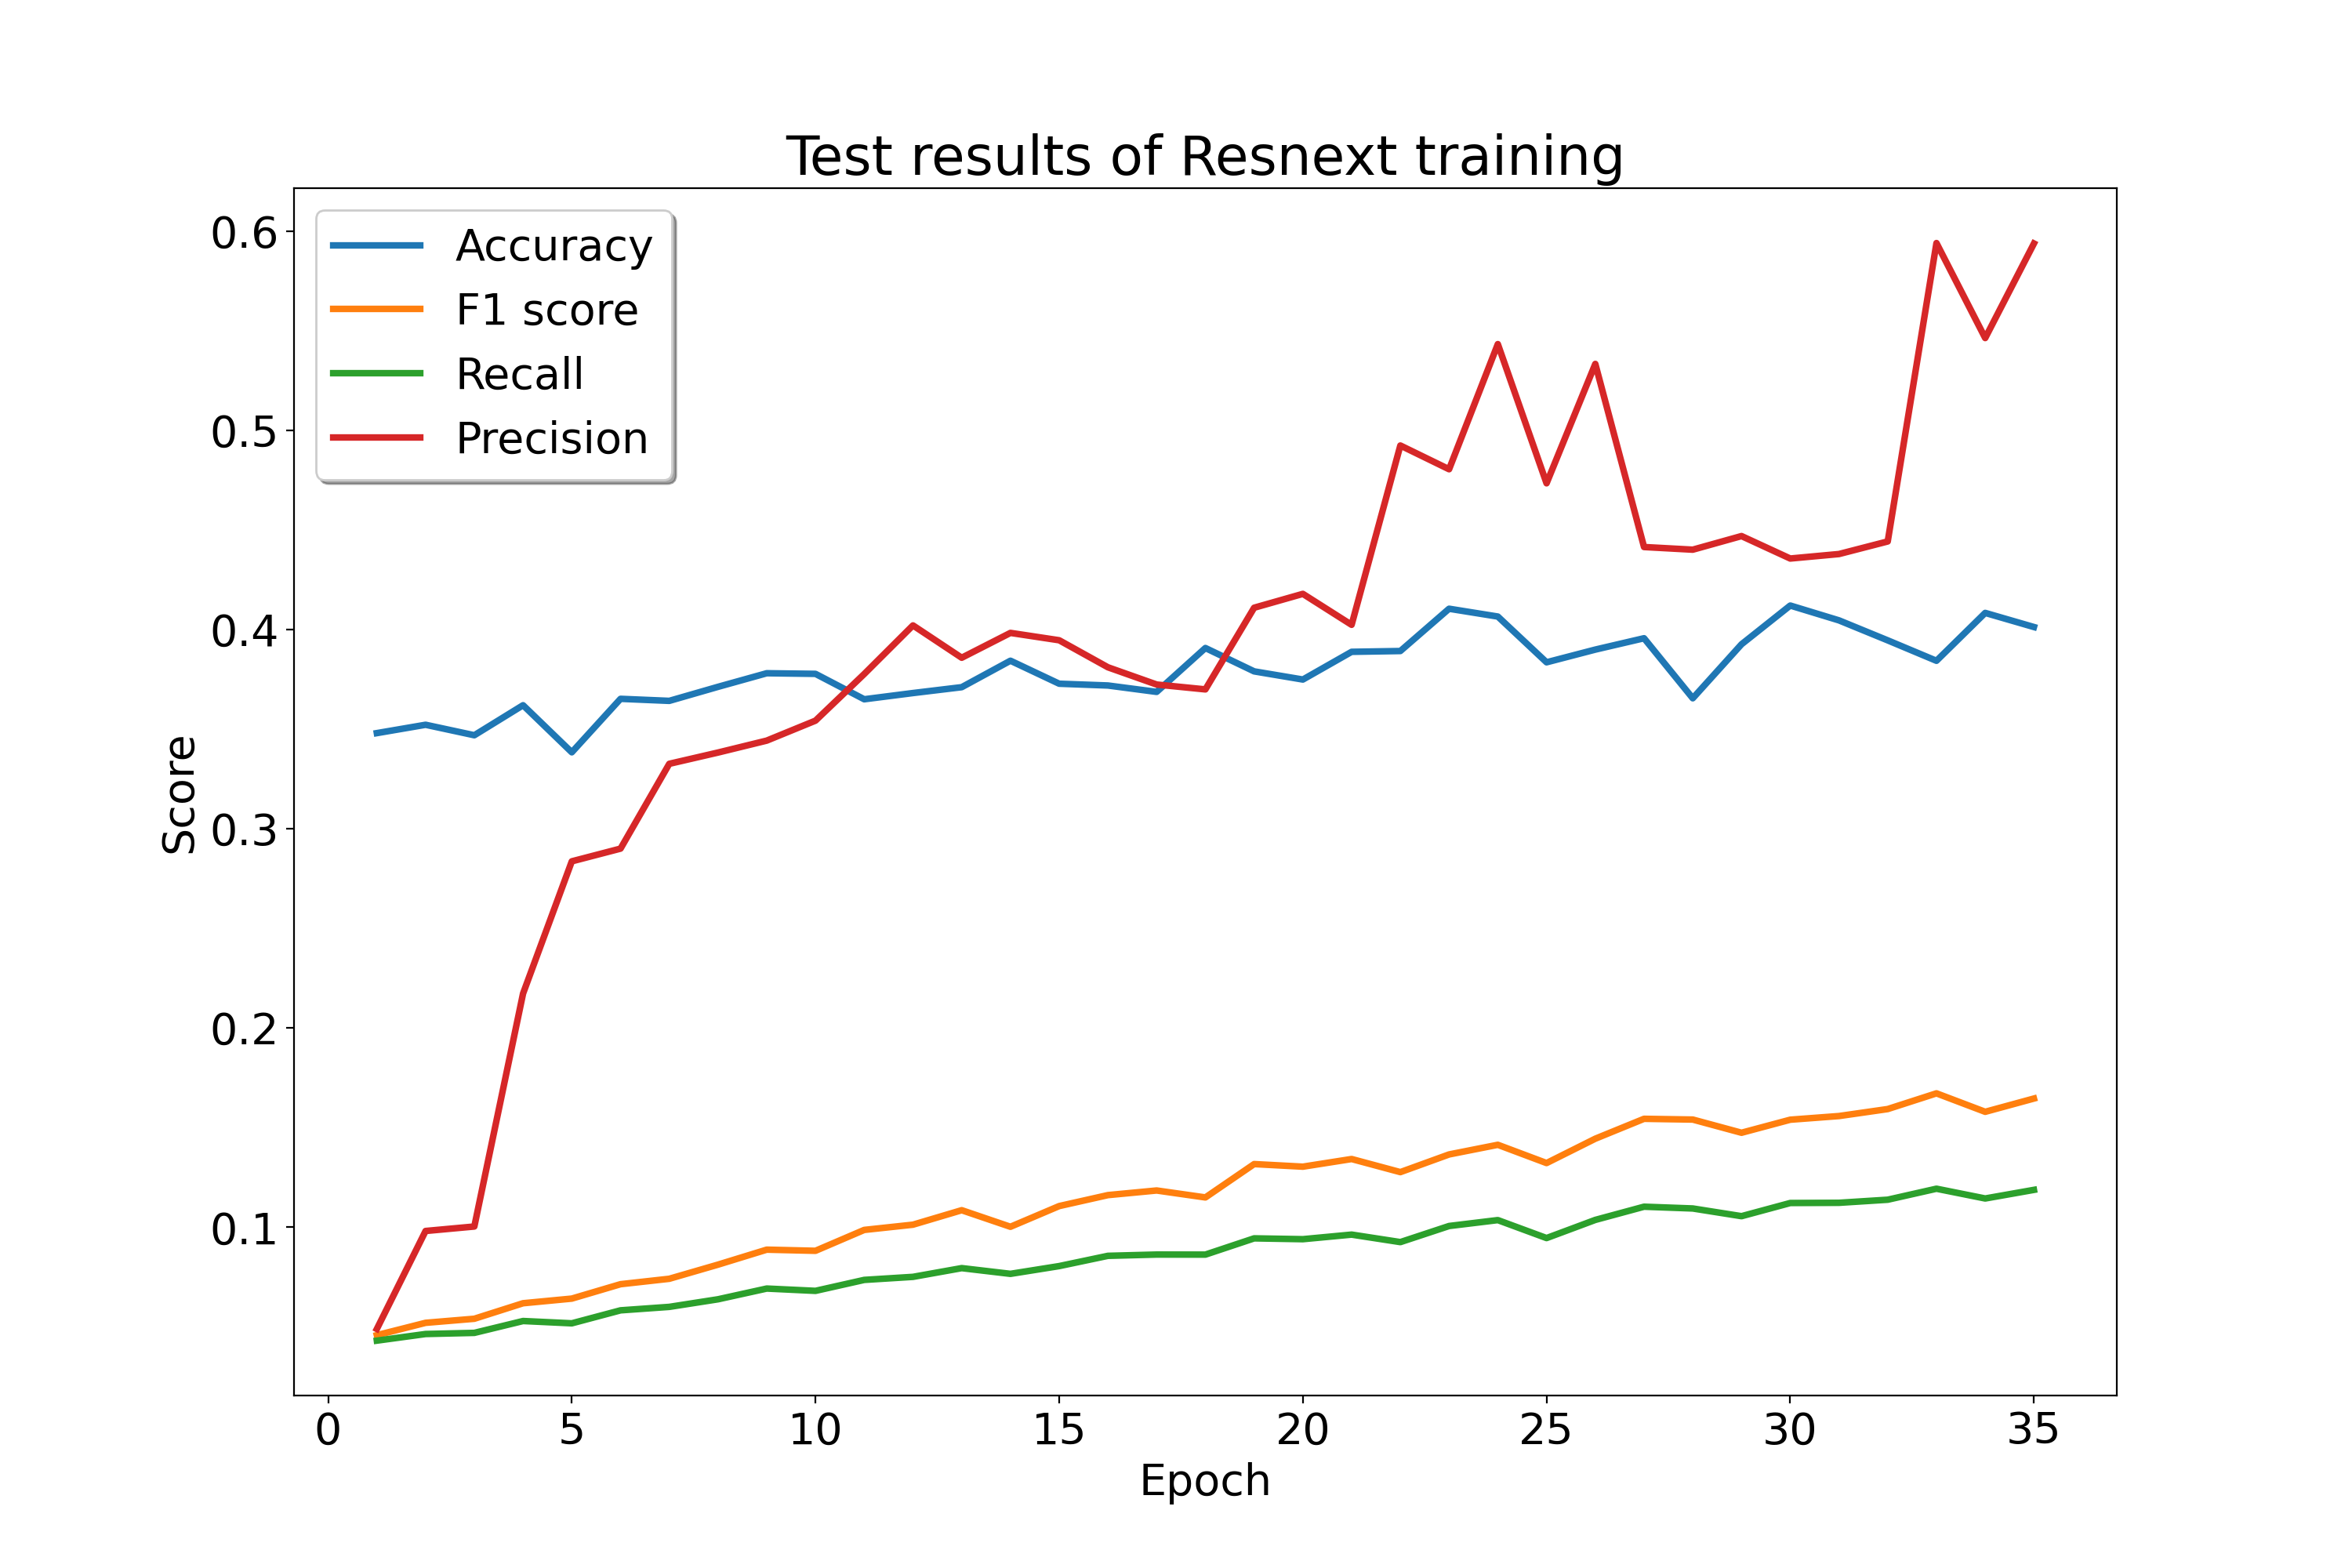
\includegraphics[width=.8\linewidth]{img/test_results_backbone_rcnn_35.png}
	\caption{ResNeXt model metrics during training}
	\label{fig:resnext_eval}
\end{figure*}

In a more refined setup we could have modified the dataloader to for example over-sample all underrepresented or on the other hand under-sample some of the dominant illness labels found in the dataset to balance the training a little more. Since again we are not really interested in the actual classification but more in the feature vectors that we can use as the Faster R-CNN backbone, we are satisfied with a final Precision of $0.59$, Recall of $0.12$, Accuracy of $0.40$ and F1 score of $0.16$. We could also certainly have trained the model further as no dramatic overfit seems to have occured yet but as will be shown in the next section, the overall results for which we need the backbone are quite satisfactory.

\section{Evaluation of Faster R-CNN and YOLO}\label{chapter:eval_rcnn_yolo}
\sectionauthor{Written by Julian Seibel}


\section{Evaluation of Study-Level Model}
\sectionauthor{Written by Torben Krieger}